\documentclass{report}

\usepackage{blindtext} % Package to generate dummy text throughout this template 
\usepackage{amsmath}
\usepackage[sc]{mathpazo} % Use the Palatino font
\usepackage[T1]{fontenc} % Use 8-bit encoding that has 256 glyphs
\usepackage{parskip}
\usepackage[english]{babel} % Language hyphenation and typographical rules
\usepackage{graphicx}

\usepackage{titling} % Customizing the title section

\usepackage{hyperref} % For hyperlinks in the PDF

%----------------------------------------------------------------------------------------
%	TITLE SECTION
%----------------------------------------------------------------------------------------

\setlength{\droptitle}{-6\baselineskip} % Move the title up

\title{Fys3120 Oblig 11} % Article title
\author{Joseph Knutson\\josephkn}



\date{\today} % Leave empty to omit a date


%----------------------------------------------------------------------------------------

\begin{document}

% Print the title
\maketitle



\section*{1a}
\begin{itemize}
\item
Problem 1A non-relativistic particle, with electric charge q and mass
m moves in a magnetic dipole field, given by the vector potential
\begin{equation}
\vec{A} = \frac{\mu_0}{4\pi r^3}(\vec{\mu}\times\vec{r}) 
\end{equation}
Show that the Lagrangian is
\begin{equation}\label{Lagrange1}
L = \frac{1}{2}m\vec{v}^2 + \frac{q\mu_0}{4\pi mr^3}\vec{\mu}\cdot\vec{l},
\end{equation}
Where $\vec{l} = m\vec{r} \times \vec{v}$
\end{itemize}

We begin with defining the Lagrangian:
$$L = T-V$$
From equation \ref{Lagrange1} it is obvious that $T=1/2mv^2$, which means, we need to prove that the potential is: 
$$V =   \frac{q\mu_0}{4\pi mr^3}\vec{\mu}\cdot\vec{l}$$
In order to prove this, we use the fact that $- q\vec{v} \cdot \vec{A} = V$:
\begin{align}
V &=  q\vec{v} \cdot \vec{A} \nonumber\\
&=\ \ \  \frac{q\mu_0}{4\pi r^3}\vec{v}(\vec{\mu}\times\vec{r})\nonumber\\
&=\ \ \  \frac{q\mu_0}{4\pi m r^3}\vec{p}(\vec{\mu}\times\vec{r})\nonumber\\
&=-\frac{q\mu_0}{4\pi m r^3}\vec{\mu}(\vec{r}\times\vec{p})\nonumber\\
&=\underline{\underline{-\frac{q\mu_0}{4\pi m r^3}\vec{\mu}\cdot\vec{l}}}\label{pot}\\\nonumber
\end{align}
%------------------------------------------------
\clearpage
\section*{1b}
\begin{itemize}
\item Particle moves in the xy-plane and $\phi$ is the angle between the x-axis and the particle's position vector $\vec{r}$. The magnetic dipole momentum, $\vec{\mu}$, has a direction along the z-axis.
Express the Lagrangian as : \begin{equation}
L = \frac{1}{2}m(\dot{r}^2+r^2\dot{\phi}^2) + \lambda\frac{\dot{\phi}}{r}\label{lambda}
\end{equation}
where \begin{equation}\lambda = q\mu_0|\vec{\mu}|/4\pi\label{mu}\end{equation}
\end{itemize}
To express the Lagrangian in equation \ref{lambda}, we start by expressing the kinetic energy in polar coordinates:
\begin{align*}
x &= r\cos{\phi}\\
y&= r\sin{\phi}\\
z&=0\\
\text{Finding velocity to express T:}\\
\vec{v} &= (\dot{x},\ \dot{y},\ 0)\\
\dot{x} &= \dot{r}\cos{\phi} - r\dot{\phi}\sin{\phi}\\
\dot{y} &= \dot{r}\sin{\phi} + r\dot{\phi}\cos{\phi}\\
\dot{z} &=0\\
\implies |\vec{v}| &= \sqrt{\dot{r}^2 + r^2\dot{\phi}^2}\\
\implies T &= \frac{1}{2}m(\dot{r}^2 + r^2\dot{\phi}^2)
\end{align*}

We now have the kinetic term of equation \ref{lambda}, but we have yet to express the potential which should be:
$V =\dot{\phi} \lambda/r$. To derive this, we need to substitute $\lambda$ from equation \ref{mu} into the potential term of our Lagrangian found in both eq. \ref{Lagrange1} and \ref{pot}.

First trick is to express the dipole momentum vector, using equation \ref{mu}:
\begin{equation} \vec{\mu} =|\vec\mu|\vec{k}\label{fag}\end{equation}
Before substituting $\lambda$ into the potential, we split the magnetic dipole vector as we did in \ref{fag}:
\begin{align}
-V &= \frac{q\mu_0}{4\pi mr^3}\vec{\mu}\cdot\vec{l} \nonumber\\
&= \frac{q\mu_0}{4\pi mr^3}|\vec{\mu}|\vec{k}\cdot\vec{l} \nonumber\\
&= \frac{\lambda}{mr^3}\vec{k}\cdot\vec{l} \nonumber\\\label{pot2}
&=|\vec{l}|\frac{\lambda}{mr^3} = |\vec r \times \vec v|\frac{m\lambda}{mr^3}=|\vec r \times \vec v|\frac{\lambda}{r^3}
\end{align}
This crossproduct requires us to look back when we derived the kinetic term:
\begin{align}
\vec r &=  (x, \ y,\ z)\nonumber\\
	   &= (r\cos \phi, \ r\sin \phi, \ 0)\\
\vec v &= (\dot x,\ \dot y, \ 0) \nonumber\\
	   &= (\dot{r}\cos{\phi} - r\dot{\phi}\sin{\phi}, \ \dot{r}\sin{\phi} + r\dot{\phi}\cos{\phi},\ 0)\\
\implies& \nonumber\\
\end{align}
\begin{align}
\vec r \times \vec v &= 
\begin{vmatrix}
\vec i&\vec j&\vec k\\
x&y&0\\
\dot x&\dot y&0\\
\end{vmatrix}
= 
\begin{vmatrix}
\vec i&\vec j&\vec k\\
x&y&0\\
\dot x&\dot y&0\\
\end{vmatrix}\\
&=(x\dot y - y \dot x)\vec k \nonumber \\
&= r\cos \phi (\dot{r}\sin{\phi} + r\dot{\phi}\cos{\phi}) -  r\sin \phi(\dot{r}\cos{\phi} - r\dot{\phi}\sin{\phi}) \\
&= r^2\dot \phi\cos^2 \phi + r^2\dot \phi\sin^2 \phi\\
&= r^2\dot \phi
\end{align}
Now that we have the crossproduct, we can insert it into our potential, back in equation \ref{pot2}
\begin{align*}-V =&|\vec r \times \vec v|\frac{\lambda}{r^3}\\
&= r^2\dot \phi\frac{\lambda}{r^3}\\&=\dot \phi\frac{\lambda}{r}\\
\end{align*}
If we look back at our kinetic term, we saw that $T = \frac{1}{2}m(\dot r^2 + r^2\phi^2)$, with this we can now express the Lagrangian on the form we set out to:
\begin{equation} L = T-V= \frac{1}{2}m(\dot r^2 + r^2\dot\phi^2) + \lambda\frac{ \dot\phi}{r}\label{swag}\end{equation}
%------------------------------------------------
\clearpage
\section*{1c}
\begin{itemize}
\item
Write Lagrange\rq{}s equation for the coordinate $r$, expressed in terms of$\dot r$, $\ddot r$ and $p_\phi$, and use the equation to find $\dot r^2$  as a function of $r$ and $p_\phi$. Compare the expression with that of the particle\rq{}s kinetic energy.
\end{itemize}

From the Lagrangian in equation \ref{swag}, we derive Lagrange\rq{}s equation for $\phi$.
Notice that the second term of the Lagrange equation is zero, which gives us the constant conjugate momentum:
\begin{align}
\frac{d}{d t} \left(\frac{\partial L}{\partial \dot\phi}   \right) - \frac{\partial L}{\partial \phi} &= 0 \nonumber\\
\nonumber\\
\frac{\partial L}{\partial \phi} &= 0\\
\frac{d}{d t} \left(\frac{\partial L}{\partial \dot\phi}   \right) &=\frac{d}{d t}\left(mr^2\dot\phi + \frac{\lambda}{r} \right)\\
\implies p_\phi &= mr^2\dot\phi + \frac{\lambda}{r}\\
\implies \dot\phi &= \frac{p_\phi r - \lambda}{mr^3}\label{phi}
\end{align}
We can use equation \ref{phi} to substitute away $\dot\phi$ out of Lagrange\rq{}s equation of $r$:
\begin{align}
\frac{d}{d t} \left(\frac{\partial L}{\partial \dot r}   \right) - \frac{\partial L}{\partial r} &= 0 \nonumber\\
\nonumber\\
\frac{d}{d t} \left(\frac{\partial L}{\partial \dot r}   \right) &= \frac{d}{d t}m\dot r = m\ddot r \\
\frac{\partial L}{\partial r} &= mr\dot \phi^2 - \lambda \frac{\dot\phi}{r^2} \ \ \ \ \ \text{     let\rq{}s substitute } \dot\phi \nonumber\\
&= mr\left(\frac{p_\phi r - \lambda}{mr^3}\right)^2 -  \frac{p_\phi r\lambda - \lambda^2}{mr^5} \nonumber \\
&= m\left(\frac{p_\phi^2 r^2 -2p_\phi r \lambda   +\lambda^2-(p_\phi r\lambda - \lambda^2)}{m^2r^5} \right) \nonumber \\
&= m\left(\frac{p_\phi^2 r^2 -3p_\phi r \lambda  }{m^2r^5} \right) \nonumber
\end{align}
Now let\rq{}s set up Lagrange\rq{}s equation since we have both derivative terms figured out:
\begin{align}
\nonumber\\
\frac{d}{d t} \left(\frac{\partial L}{\partial \dot r}   \right) - \frac{\partial L}{\partial r} =& m\left(\ddot r - \frac{p_\phi^2 r^2 +3p_\phi r \lambda  }{m^2r^5}   \right)  \\
\implies  \ddot r =& \frac{p_\phi^2 r^2 - 3p_\phi r \lambda  }{m^2r^5} \\
\implies  \dot r =& \frac{p_\phi^2}{m^2} \int \frac{1}{r^3}dt   - 3\lambda\frac{p_\phi}{m^2}\int \frac{1}{r^4} dt \label{swag2}
\end{align}
Since our goal is to express $\dot r ^2$ we need to integrate $\ddot r$, but first we gotta substitute $dt$ out of the equation.
$$dt = \frac{dr}{dr} dt = \frac{dt}{dr} dr = \frac{1}{\dot r} dr$$
Let\rq{}s substitute this into equation \ref{swag2} to solve it:
\begin{align}
 \dot r &= \frac{p_\phi^2}{m^2} \int \frac{1}{r^3}dt   - 3\lambda\frac{p_\phi}{m^2}\int \frac{1}{r^4} dt  \nonumber\\
 \dot r &= \frac{p_\phi^2}{m^2} \int \frac{1}{\dot r r^3}dr   - 3\lambda\frac{p_\phi}{m^2}\int \frac{1}{\dot r r^4} dr  \label{swag3}
\end{align}
Let\rq{}s do a cool trick and multiply with $\dot r$  on both sides of  equation \ref{swag3}:
\begin{align}
 \dot r^2 =& \frac{p_\phi^2}{m^2} \int \frac{1}{ r^3}dr   - 3\lambda\frac{p_\phi}{m^2}\int \frac{1}{ r^4} dr  \nonumber\\
\nonumber\\
 =& -\frac{p_\phi^2}{2m^2}  \frac{1}{ r^2}   + \lambda\frac{p_\phi}{m^2} \frac{1}{ r^3}   \\
=& \underline{\underline{\frac{p_\phi}{2m^2r^2}( \frac{2\lambda}{r} -  p_\phi) }}\\
%&= \frac{mr^2\dot\phi + \frac{\lambda}{r}}{2m^2r^2}( \frac{2\lambda}{r} - (mr^2\dot\phi + \frac{\lambda}{r}))\\
%&= \frac{\dot \phi}{2} + \frac{\frac{\lambda}{r}}{2m^2r^2}  ( \frac{\lambda}{r} -  mr^2\dot\phi)\\
%&= \frac{\dot \phi}{2} + \frac{\lambda^2}{2m^2r^4}  -  \frac{\lambda mr^2\dot\phi}{2m^2r^3}\\
%&= \frac{\dot \phi}{2} + \frac{\lambda^2}{2m^2r^4}  -  \frac{\lambda \dot\phi}{2r}\\
%\\
\nonumber\\
\text{Comparing this mess with the kinetic}&\text{ energy is completely lost on me.}\nonumber\\ 
\text{ Perhaps I made a miscalculation.}\nonumber \ \ \ \ \   \ \ &\\ 
T =& \frac{1}{2}m(\dot r^2 + r^2\dot\phi^2)
\end{align}
\clearpage
\section*{2 Relatively cool circuit}
Figure \ref{loop} shows a rectangular current loop ABCD. In the loop\rq{}s rest frame, S, the loop has length a in the x direction and width b in the y direction, the current is I and the charge density is zero. We remind you of the following general definitions of the electric dipole moment $\vec p$, and the magnetic dipole moment $\vec m$, for a given current distribution: 
\begin{equation}
\vec p = \int \vec r \rho(\vec r) d^3r \label{electric}
\end{equation}
\begin{equation}
\vec m = \frac{1}{2}\int (\vec r \times \vec j(\vec r)) d^3r \label{magnetic}
\end{equation}

\begin{figure}
\centering
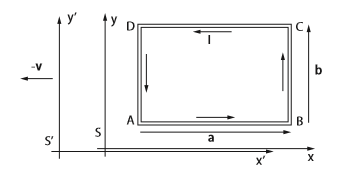
\includegraphics{loop}
\caption{Current loop ABCD of length $a$ and width $b$. Zero charge density.}
\label{loop}
\end{figure}
\section*{2a}
\begin{itemize}
\item
Show that the electric dipole moment is zero in the loop\rq{}s restframe. Show that the magnetic dipole moment is $\vec m = I\vec a \times \vec b$ where $I = j\Delta$. $\Delta $ is the cross sectional area of the conductor. 
\end{itemize}
Because our conductor is without charge density in the S frame ($\rho = 0$), the integral in equation \ref{electric}, the electric dipole momentum, equals zero.

In order to determine the magnetic dipole momentum we must express $\vec r \times \vec j$.
\end{document}
